% System architecture of protocol v2, laid out for one IEEE column (86 mm).
\documentclass[tikz,border=1pt]{standalone}
\usepackage{newtxtext,newtxmath}
\usetikzlibrary{arrows.meta,fit,backgrounds}
\newcommand{\sm}{\fontsize{6}{7}\selectfont}
\begin{document}
\scriptsize
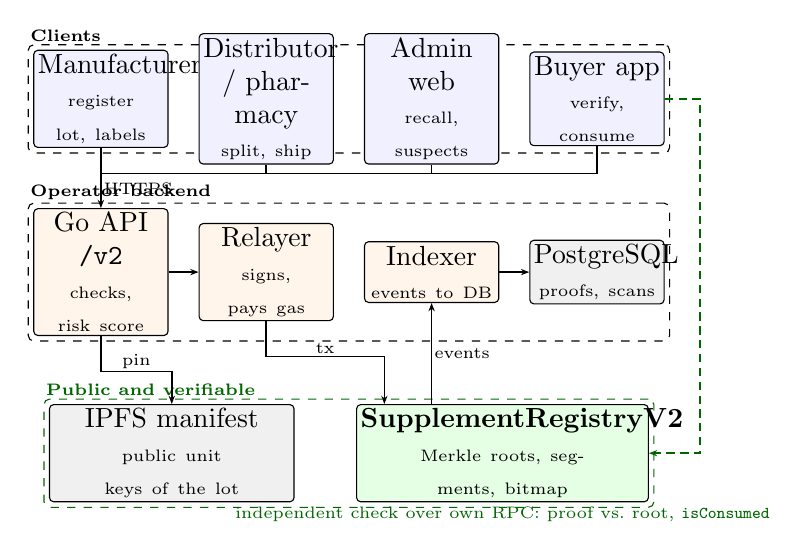
\begin{tikzpicture}[
  x=1mm, y=1mm,
  >={Stealth[length=3pt]},
  box/.style={draw, rounded corners=1.5pt, align=center, inner sep=1.5pt, minimum height=7.5mm, text width=16mm, fill=white},
  app/.style={box, fill=blue!6},
  svc/.style={box, fill=orange!8},
  store/.style={box, fill=gray!12},
  chain/.style={box, fill=green!10, text width=36mm},
  group/.style={draw, dashed, rounded corners=2pt, inner sep=1.8pt},
  glabel/.style={font=\sm\bfseries, inner sep=0.8pt, anchor=south west},
  lbl/.style={font=\sm, inner sep=0.8pt},
  flow/.style={->, semithick},
  check/.style={->, semithick, densely dashed, green!40!black},
]
  \node[app] (mfr)   at (9,0)  {Manufacturer\\{\sm register lot, labels}};
  \node[app] (dist)  at (30,0) {Distributor / pharmacy\\{\sm split, ship}};
  \node[app] (admin) at (51,0) {Admin web\\{\sm recall, suspects}};
  \node[app] (buyer) at (72,0) {Buyer app\\{\sm verify, consume}};

  \node[svc] (api)   at (9,-22)  {Go API \texttt{/v2}\\{\sm checks, risk score}};
  \node[svc] (relay) at (30,-22) {Relayer\\{\sm signs, pays gas}};
  \node[svc] (idx)   at (51,-22) {Indexer\\{\sm events to DB}};
  \node[store] (pg)  at (72,-22) {PostgreSQL\\{\sm proofs, scans}};

  \node[store, text width=30mm] (ipfs) at (18,-45) {IPFS manifest\\{\sm public unit keys of the lot}};
  \node[chain] (reg) at (60,-45) {\textbf{SupplementRegistryV2}\\{\sm Merkle roots, segments, bitmap}};

  \begin{scope}[on background layer]
    \node[group, fit=(mfr)(buyer)] (gc) {};
    \node[group, fit=(api)(pg)] (gb) {};
    \node[group, draw=green!40!black, fit=(ipfs)(reg)] (gp) {};
  \end{scope}
  \node[glabel] at (gc.north west) {Clients};
  \node[glabel] at (gb.north west) {Operator backend};
  \node[glabel, text=green!40!black] at (gp.north west) {Public and verifiable};

  % clients reach the API over HTTPS
  \foreach \c in {mfr, dist, admin, buyer} \draw[semithick] (\c.south) -- (\c.south |- 0,-9.5);
  \draw[semithick] (9,-9.5) -- (72,-9.5);
  \draw[flow] (9,-9.5) -- node[lbl, right, pos=0.45] {HTTPS} (api.north);

  \draw[flow] (api) -- (relay);
  \draw[flow] (idx) -- (pg);
  \draw[flow] (api.south) -- ++(0,-4.5) -| node[lbl, above, pos=0.25] {pin} (ipfs.north);
  \draw[flow] (relay.south) -- ++(0,-4.5) -| node[lbl, above, pos=0.25] {tx} (45,0 |- reg.north);
  \draw[flow] (51,0 |- reg.north) -- node[lbl, right] {events} (idx.south);

  % the buyer's app re-checks the API's answer against the chain
  \draw[check] (buyer.east) -- ++(4.5,0) |- (reg.east);
  \node[lbl, text=green!40!black, align=center, anchor=north] at (60,-51.5)
    {independent check over own RPC: proof vs.\ root, \texttt{isConsumed}};
\end{tikzpicture}
\end{document}
